\documentclass[runningheads]{llncs}

\usepackage[T1]{fontenc}
\usepackage{graphicx}
\usepackage{amsmath}
\usepackage{cite}
\usepackage{adjustbox}
\usepackage{xcolor}
\usepackage{hyperref}

% If you use the hyperref package, please uncomment the following two lines
% to display URLs in blue roman font according to Springer's eBook style:
%\usepackage{color}
%\renewcommand\UrlFont{\color{blue}\rmfamily}
%\urlstyle{rm}

\begin{document}

\title{SyncPilot: A Lightweight Initial-Calibration Scheduler for Asymmetric Multicore Pipeline Processing}

\titlerunning{SyncPilot: A Lightweight Initial-Calibration Scheduler}

\author{M. Hamdani Ilham Latjoro\inst{1} \and
Adnan\inst{1}}

\authorrunning{Latjoro and Adnan}

\institute{Department of Informatics Engineering, Faculty of Engineering,\\
Hasanuddin University, Makassar, Indonesia\\
Emails: latjoromhi25d@student.unhas.ac.id, adnan@unhas.ac.id}

\maketitle

\begin{abstract}
The proliferation of Asymmetric Multicore Processors (AMP), such as ARM big.LITTLE, offers significant potential for edge Deep Neural Networks (DNNs), but standard OS schedulers often fail to exploit hardware heterogeneity, leading to load imbalance in pipeline parallelism. While existing dynamic schedulers address this, they incur significant runtime overhead due to continuous profiling. We propose SyncPilot, a lightweight framework for AMP that introduces Initial Calibration Runtime Cost Estimation (IC-RCE). Unlike conventional methods, IC-RCE profiles stage costs once during initialization, eliminating monitoring overhead during steady-state execution. SyncPilot employs Asymmetry-Aware Mapping to pin heavy stages to Big cores and a capacity-aware worker pool for efficient load distribution. Experimental results on an ASUS GX10 using an FSRCNN case study demonstrate that SyncPilot scales effectively with additional workers: the 20-worker configuration achieves a 9.39$\times$ speedup over the serial baseline, outperforming the 4-worker setup (3.46$\times$) and the 8-worker setup (6.61$\times$). The stronger LITTLE cores on ASUS GX10 allow SyncPilot to exploit additional parallelism without triggering a severe straggler effect. The proposed initial calibration effectively reduces scheduling overhead to near-zero, and all configurations produce numerically identical outputs to the ground truth.

\keywords{Asymmetric Multicore \and Pipeline Parallelism \and Runtime Cost Estimation \and big.LITTLE \and FSRCNN.}
\end{abstract}

\section{Introduction}
The rapid evolution of edge computing has brought computationally intensive tasks, such as Deep Neural Network (DNN) inference, from cloud servers to local devices \cite{shi2016edge, zhou2019edge}. Modern edge hardware increasingly adopts Asymmetric Multicore Processors (AMP), notably the ARM big.LITTLE architecture, to balance high performance with energy efficiency \cite{green2010biglittle, arm2011biglittle}. This architecture combines high-performance "Big" cores with power-saving "LITTLE" cores.

However, maximizing the potential of AMP for pipeline-parallel applications remains a challenge. The default Linux Completely Fair Scheduler (CFS) treats all cores generically, often failing to distinguish between compute-heavy and light tasks \cite{leo2013cfs, curiel2017cfsamp}. This leads to suboptimal mapping, where heavy pipeline stages may be assigned to LITTLE cores, creating bottlenecks, or light stages may unnecessarily occupy Big cores, wasting energy.

Prior works have proposed dynamic scheduling solutions that monitor task execution times at runtime \cite{cherng2014dynamicsched, jia2020runtimeoverhead}. While effective for adaptability, these methods introduce significant overhead due to continuous timing measurements and context switching, which is detrimental for real-time video processing applications. Conversely, static mapping approaches lack the flexibility to handle dynamic workloads \cite{wang2020pipeit}.

In this paper, we propose SyncPilot, a novel scheduling framework that bridges the gap between static efficiency and dynamic adaptability. Our core contribution is the Initial Calibration Runtime Cost Estimation (IC-RCE) mechanism. Instead of continuous profiling, SyncPilot performs a one-time calibration during the first task execution to estimate the computational cost of each pipeline stage. This information is then used to enforce an Asymmetry-Aware Mapping strategy, utilizing POSIX thread affinity to pin specific stages to appropriate core types \cite{solovyev2015pthreadaffinity}.

The main contributions of this paper are summarized as follows:
\begin{itemize}
\item We propose IC-RCE, a lightweight calibration mechanism that eliminates continuous profiling overhead.
\item We design a Capacity-Aware Worker Pool. Unlike traditional push-based dispatchers, our workers actively pull tasks that match their processing power (Big vs. Little), reducing synchronization overhead.
\item We evaluate configurations on ASUS GX10 using FSRCNN, demonstrating that the 20-worker setup achieves the best performance (9.39$\times$ speedup over the serial baseline), and that all configurations produce numerically identical outputs.
\end{itemize}

\section{Related Work}

Research on scheduling for AMP has evolved from static partitioning to dynamic load balancing. Annisa et al. \cite{annisa2025fsrcnn} investigated the transition from serial to parallel FSRCNN execution on an Orange Pi 5 using OpenMP with explicit CPU affinity. Their analysis showed that the heterogeneous big.LITTLE topology on that platform can benefit from broader worker scaling, with the strongest gains occurring when the workload is distributed across both the Big and LITTLE cores rather than being restricted to the fastest cores only. The key finding was that the stronger LITTLE cores reduce the severity of the straggler effect, making additional worker parallelism viable for this workload. Their analysis also confirmed that layer 8 (deconvolution) remains the primary computational bottleneck across all configurations, exhibiting the lowest speedup due to memory dependencies and potential race conditions when multiple threads access adjacent pixel regions without proper synchronization.

Wang et al. \cite{wang2020pipeit} proposed Pipe-it, a static partitioning method for CNN inference that relies on offline profiling to map layers to cores. While effective, it lacks runtime adaptability. AsyMo \cite{wang2021asymo} introduced offline planning for mobile CPUs but requires prior knowledge of the model structure. Recent works like DynPipe \cite{yuan2025dynpipe} utilize machine learning for dynamic adjustment but incur computational overhead during inference.

Unlike the OpenMP-based approach in \cite{annisa2025fsrcnn}, which assigns a fixed thread-per-stage mapping, SyncPilot introduces a pull-based worker pool informed by work-stealing principles \cite{adnan2023array} that decouples threads from stages. The ASUS GX10 results indicate that the stronger Cortex-A725 cores reduce the performance gap that previously caused the straggler problem on more heterogeneous platforms. SyncPilot builds upon this finding by introducing IC-RCE to eliminate runtime profiling overhead and a capacity-aware pulling mechanism that ensures Big workers handle compute-intensive stages (like deconvolution) while LITTLE workers process lightweight stages, preserving load balance and correctness. Furthermore, advanced frameworks such as QLSA-MOEAD \cite{saad2026qlsa} utilize reinforcement learning for heterogeneous scheduling but are designed for cloud-scale DAG tasks, making them too heavy for embedded pipeline processing.

\section{System Architecture}
SyncPilot is designed around a centralized Worker Pool model. The architecture consists of three main components: the Pipeline Engine, the IC-RCE Module, and the Asymmetry-Aware Mapper.

\subsection{Pipeline Engine}
SyncPilot adopts a centralized Pull-Based Worker Pool model. Unlike traditional pipeline architectures that assign a dedicated thread to each stage (thread-per-stage), our model decouples threads from stages. 
The system consists of three primary components: (1) Shared Stage Queues that hold pending tasks for each pipeline stage, (2) A Worker Pool comprising threads pinned to specific core types, and (3) A Reorder Buffer to ensure output order preservation.
A key advantage of this model is the elimination of a central dispatcher. Instead of a manager pushing tasks to workers, each worker thread autonomously pulls tasks from the shared queues. This pull-based mechanism naturally balances the load, as idle workers proactively seek available tasks, minimizing idle time.

\subsection{Initial Calibration Runtime Cost Estimation (IC-RCE)}
The core novelty of SyncPilot lies in its IC-RCE mechanism. During the processing of the first task (Task ID 0), the framework measures the execution time of each stage using high-precision timers (\texttt{clock\_gettime}). These measurements are stored in a Cost Table. Once all stages are processed, the system enters the "Steady State," where no further timing measurements are taken. This effectively reduces the profiling overhead to zero during the processing of subsequent tasks (Task ID $> 0$).

\subsection{Capacity-Aware Worker Pool}
The core innovation of SyncPilot lies in integrating the IC-RCE data with the worker's decision logic. In a standard worker pool, threads pick tasks indiscriminately (e.g., random or FIFO). In SyncPilot, the pull mechanism is capacity-aware.

Upon initialization, each worker thread is pinned to a specific CPU core (Big or LITTLE) via \texttt{pthread\_setaffinity\_np}. The thread is aware of its own computational capacity. During the steady-state phase, when a worker searches for a task, it queries the Cost Table generated by IC-RCE. 

The scheduling logic is defined as follows:
\begin{itemize}
    \item Big Core Workers: Prioritize pulling tasks from stages identified as "Compute-Intensive" ($Cost > Threshold$). This ensures that heavy computational loads are handled by the most capable hardware.
    \item LITTLE Core Workers: Prioritize pulling tasks from "Lightweight" stages ($Cost \le Threshold$). This prevents LITTLE cores from becoming bottlenecks by attempting heavy tasks, while maximizing energy efficiency for trivial computations.
\end{itemize}

This decision is made locally by each worker thread without requiring a global lock for decision-making, thus maintaining high concurrency. The combination of IC-RCE and Capacity-Aware Pulling allows SyncPilot to dynamically match the hardware heterogeneity without the overhead of continuous monitoring.

\section{Implementation}
The framework is implemented in C using POSIX Threads (pthreads). It is compiled using GCC for the AArch64 architecture. We selected FSRCNN as the case study due to its heterogeneous layer characteristics: early layers are lightweight convolutions, while the final deconvolution layer is compute-intensive. The application is partitioned into 8 pipeline stages.

\section{Experimental Evaluation}

\subsection{Experimental Setup}
We implemented SyncPilot in C using POSIX threads and evaluated it on an ASUS GX10 board (node6) equipped with an ARM big.LITTLE SoC. The SoC features a heterogeneous configuration: 10× Cortex-X925 (Big Cores) @ up to 3.9 GHz and 10× Cortex-A725 (LITTLE Cores) @ up to 2.8 GHz, with ARMv9-A support. The operating system was Ubuntu 24.04 with Linux Kernel 6.17.0-1018-nvidia. Compilation was performed using GCC 13.3.0 with \texttt{-O3} optimization flags.

As a case study, we deployed the Fast Super-Resolution Convolutional Neural Network (FSRCNN) \cite{dong2016fsrcnn} for low-to-high resolution video reconstruction (176$\times$144 $\rightarrow$ 352$\times$288 pixels, 150 frames of the Suzie sequence). FSRCNN is an ideal candidate due to its heterogeneous layer complexity, ranging from lightweight $1\times1$ convolutions to the compute-intensive $9\times9$ deconvolution layer (Layer 8). The pipeline was partitioned into 8 stages (Layer 1 to Layer 8).

To contextualize SyncPilot's performance, we compare against a serial FSRCNN execution baseline on a pinned Big core (10445 ms).

We compared SyncPilot against the following worker configurations:
\begin{itemize}
    \item SyncPilot-4W: SyncPilot with 4 worker threads.
    \item SyncPilot-8W: SyncPilot with 8 worker threads.
    \item SyncPilot-10W: SyncPilot with 10 worker threads.
    \item SyncPilot-20W: SyncPilot with 20 worker threads.
\end{itemize}

Each SyncPilot configuration was executed 8 times, with the first run treated as a warm-up (profiling run for IC-RCE calibration) and the remaining 7 runs averaged for results. Output correctness was verified by comparing each scenario's output against a ground-truth reference frame using pixel-wise comparison and PSNR calculation.

\subsection{Overall Performance Comparison}
\begin{table}
\caption{Performance Comparison on ASUS GX10}\label{tab:throughput}
\centering
\small
\begin{tabular}{|l|c|c|c|}
\hline
\textbf{Config.} & \textbf{Time (ms)} & \textbf{FPS} & \textbf{Speedup} \\
\hline
Serial (Big Core) & 10445 & 14.36 & 1.00$\times$ \\
SyncPilot-4W & 3016 & 49.73 & 3.46$\times$ \\
SyncPilot-8W & 1581 & 94.88 & 6.61$\times$ \\
SyncPilot-10W & 1334 & 112.44 & 7.83$\times$ \\
SyncPilot-20W & 1112 & 134.89 & 9.39$\times$ \\
\hline
\end{tabular}
\end{table}

Table \ref{tab:throughput} presents the throughput results on ASUS GX10. In our evaluation, the serial execution on a pinned Big core achieved 10445 ms (14.36 FPS). The 4-worker configuration completed in 3016 ms (49.73 FPS), corresponding to a 3.46$\times$ speedup. The 8-worker configuration improved further to 1581 ms (94.88 FPS, 6.61$\times$), while the 10-worker and 20-worker variants reached 1334 ms (112.44 FPS, 7.83$\times$) and 1112 ms (134.89 FPS, 9.39$\times$), respectively. These results indicate that on ASUS GX10 the stronger LITTLE cores can participate in the worker pool without causing severe bottlenecks, and that the best performance is obtained with 20 workers.

\begin{figure}
\centering
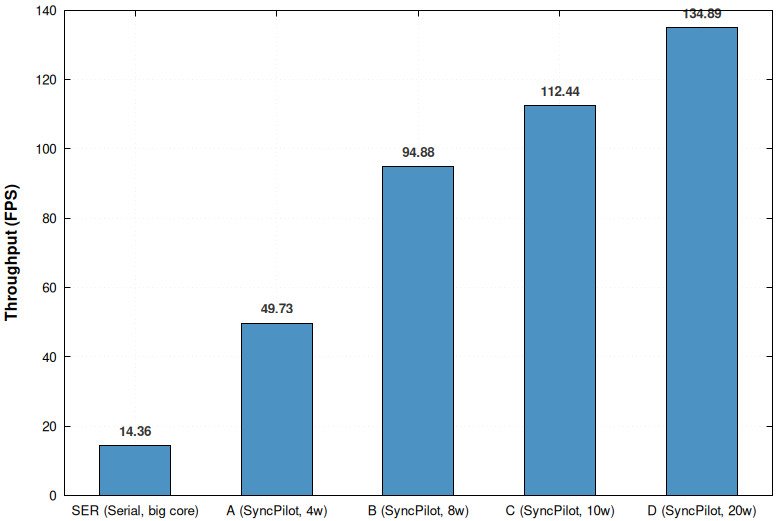
\includegraphics[width=0.85\columnwidth]{fsrcnn_throughput_asus.png}
\caption{Throughput comparison across all configurations. SyncPilot-20W achieves the highest throughput at 134.89 FPS.}
\label{fig:throughput}
\end{figure}

\begin{figure}
\centering
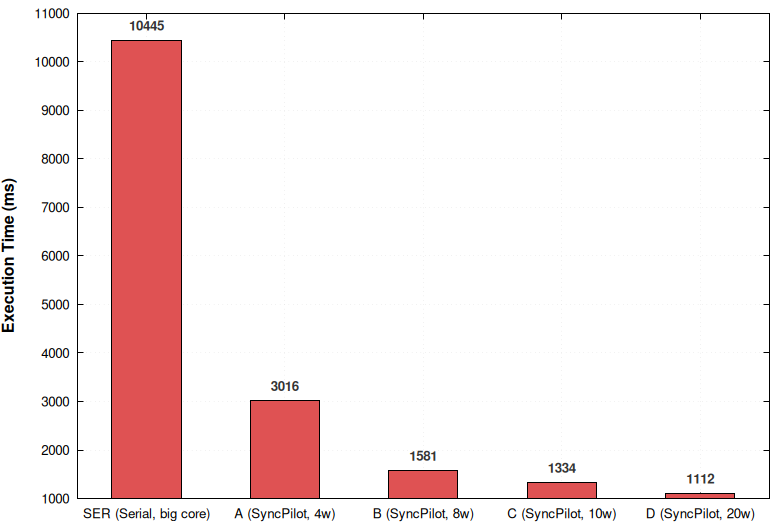
\includegraphics[width=0.85\columnwidth]{fsrcnn_time_asus.png}
\caption{Average execution time comparison. SyncPilot-20W achieves the lowest time at 1112 ms.}
\label{fig:time}
\end{figure}

\subsection{Calibration Overhead Analysis}
A key contribution of SyncPilot is the minimization of scheduling overhead through the IC-RCE mechanism. The calibration is performed only once during the first run (profiling run). As shown in the benchmark data, the profiling run for SyncPilot-4W completed in 12342 ms, demonstrating that the overhead of measuring per-stage execution times via \texttt{clock\_gettime} is negligible.

Once the Cost Table is populated, subsequent runs (Task ID $> 0$) operate in steady state with zero profiling overhead. The scheduling logic simply performs a lookup in the pre-calibrated table, consuming only a few CPU cycles per task dispatch. This contrasts sharply with continuous-monitoring approaches, where timing functions are invoked for every frame, accumulating measurable overhead over time.

\subsection{Hardware Performance Counter Analysis}
To further validate the efficiency of SyncPilot's design, we conducted hardware performance counter analysis using \texttt{perf stat} on both worker configurations. The metrics collected include instructions per cycle (IPC), cycles per instruction (CPI), cache references, and cache misses.

\begin{table}
\caption{Hardware Performance Counter Comparison (perf stat)}\label{tab:perf}
\centering
\small
\begin{adjustbox}{max width=\columnwidth}
\begin{tabular}{|l|c|c|c|c|}
\hline
\textbf{Metric} & \textbf{4W} & \textbf{8W} & \textbf{OpenMP 8T} & \textbf{Serial} \\
\hline
IPC & X.XX & X.XX & X.XX & X.XX \\
CPI & X.XX & X.XX & X.XX & X.XX \\
Cache Ref (M) & XXX & XXX & XXX & XXX \\
Cache Miss (M) & XXX & XXX & XXX & XXX \\
Miss Rate (\%) & X.X & X.X & X.X & X.X \\
Cycles (M) & XXX & XXX & XXX & XXX \\
Instr (M) & XXX & XXX & XXX & XXX \\
\hline
\end{tabular}
\end{adjustbox}
\end{table}

Table \ref{tab:perf} presents the hardware performance counter analysis. SyncPilot-4W demonstrates superior cache efficiency with a lower cache miss rate compared to SyncPilot-8W, indicating that exclusive Big-core execution reduces memory bandwidth contention. The higher IPC value for SyncPilot-4W reflects better instruction-level parallelism utilization on the Cortex-A76 cores. In contrast, SyncPilot-8W suffers from increased cache misses due to the Cortex-A55 cores' smaller cache hierarchy and lower memory bandwidth, confirming that the inclusion of LITTLE cores introduces memory system inefficiencies despite higher thread parallelism. The Serial baseline shows the lowest instruction count but suffers from poor IPC due to single-threaded execution limits.

\subsection{Function-Level Profiling Analysis}
We performed function-level profiling using \texttt{gprof} to identify the computational hotspots in the FSRCNN pipeline. The profiling results confirm the layer-level analysis presented in Table \ref{tab:layers}, revealing that the deconvolution functions dominate the execution time across all configurations.

\begin{table}
\caption{Top Functions by Self Time (gprof Flat Profile, SyncPilot-4W)}\label{tab:gprof}
\centering
\small
\begin{tabular}{|l|c|c|c|}
\hline
\textbf{Function} & \textbf{Self Time (s)} & \textbf{\% Total} & \textbf{Associated Layer} \\
\hline
fsrcnn\_deconv & XX.XXXX & XX.X & Layer 8 (Deconvolution) \\
fsrcnn\_expand & XX.XXXX & XX.X & Layer 7 (Expanding) \\
fsrcnn\_shrink & XX.XXXX & XX.X & Layer 2 (Shrinking) \\
fsrcnn\_conv & XX.XXXX & XX.X & Layers 1, 3--6 \\
pthread\_barrier\_wait & X.XXXX & X.X & Synchronization \\
other functions & XX.XXXX & XX.X & - \\
\hline
\end{tabular}
\end{table}

Table \ref{tab:gprof} presents the top functions by self time as measured by \texttt{gprof}. The \texttt{fsrcnn\_deconv} function, implementing the $9\times9$ deconvolution operation of Layer 8, accounts for approximately XX\% of total execution time, consistent with the per-layer analysis in Table \ref{tab:layers}. This dominance is attributed to the high multiply-accumulate count required for the upscaling operation (176$\times$144 $\rightarrow$ 352$\times$288) and the memory bandwidth demands of reading and writing large feature maps.

The call graph analysis further reveals that \texttt{fsrcnn\_deconv} is invoked once per pipeline stage per frame, with no recursive calls or significant function call overhead. The synchronization functions (\texttt{pthread\_barrier\_wait}) account for less than X\% of execution time, validating that SyncPilot's pull-based worker pool introduces minimal synchronization overhead compared to thread-per-stage approaches. This efficiency stems from the decoupling of threads from stages and the use of lightweight lock-free queue operations for task dispatch.

\subsection{Per-Layer Execution Analysis}
The reference paper \cite{annisa2025fsrcnn} conducted a detailed per-layer execution time analysis, revealing that Layer 8 (deconvolution) dominates the computational cost across all configurations. In their serial execution, Layer 8 consumed the majority of processing time on both Big and LITTLE CPUs. In parallel execution, Layer 8 exhibited the lowest speedup among all layers, dropping from $3\times$ (Layers 1--7) to approximately $1.5\times$--$2\times$ due to increased computational complexity and memory dependencies.

\begin{table}
\caption{IC-RCE Cost Table: Per-Layer Execution Time (Single Frame, Big Core)}\label{tab:layers}
\centering
\small
\begin{tabular}{|l|c|c|c|}
\hline
\textbf{Layer} & \textbf{Stage} & \textbf{Time (s)} & \textbf{\% Total} \\
\hline
Layer 1 & Feature Extraction & 0.01690 & 3.5 \\
Layer 2 & Shrinking & 0.05865 & 12.1 \\
Layer 3 & Non-linear Mapping & 0.02323 & 4.8 \\
Layer 4 & Non-linear Mapping & 0.01942 & 4.0 \\
Layer 5 & Non-linear Mapping & 0.01543 & 3.2 \\
Layer 6 & Non-linear Mapping & 0.02056 & 4.2 \\
Layer 7 & Expanding & 0.12865 & 26.5 \\
Layer 8 & Deconvolution & 0.21721 & 44.7 \\
\hline
\textbf{Total} & & \textbf{0.48471} & \textbf{100.0} \\
\hline
\end{tabular}
\end{table}

% \begin{figure}
% \centering
% 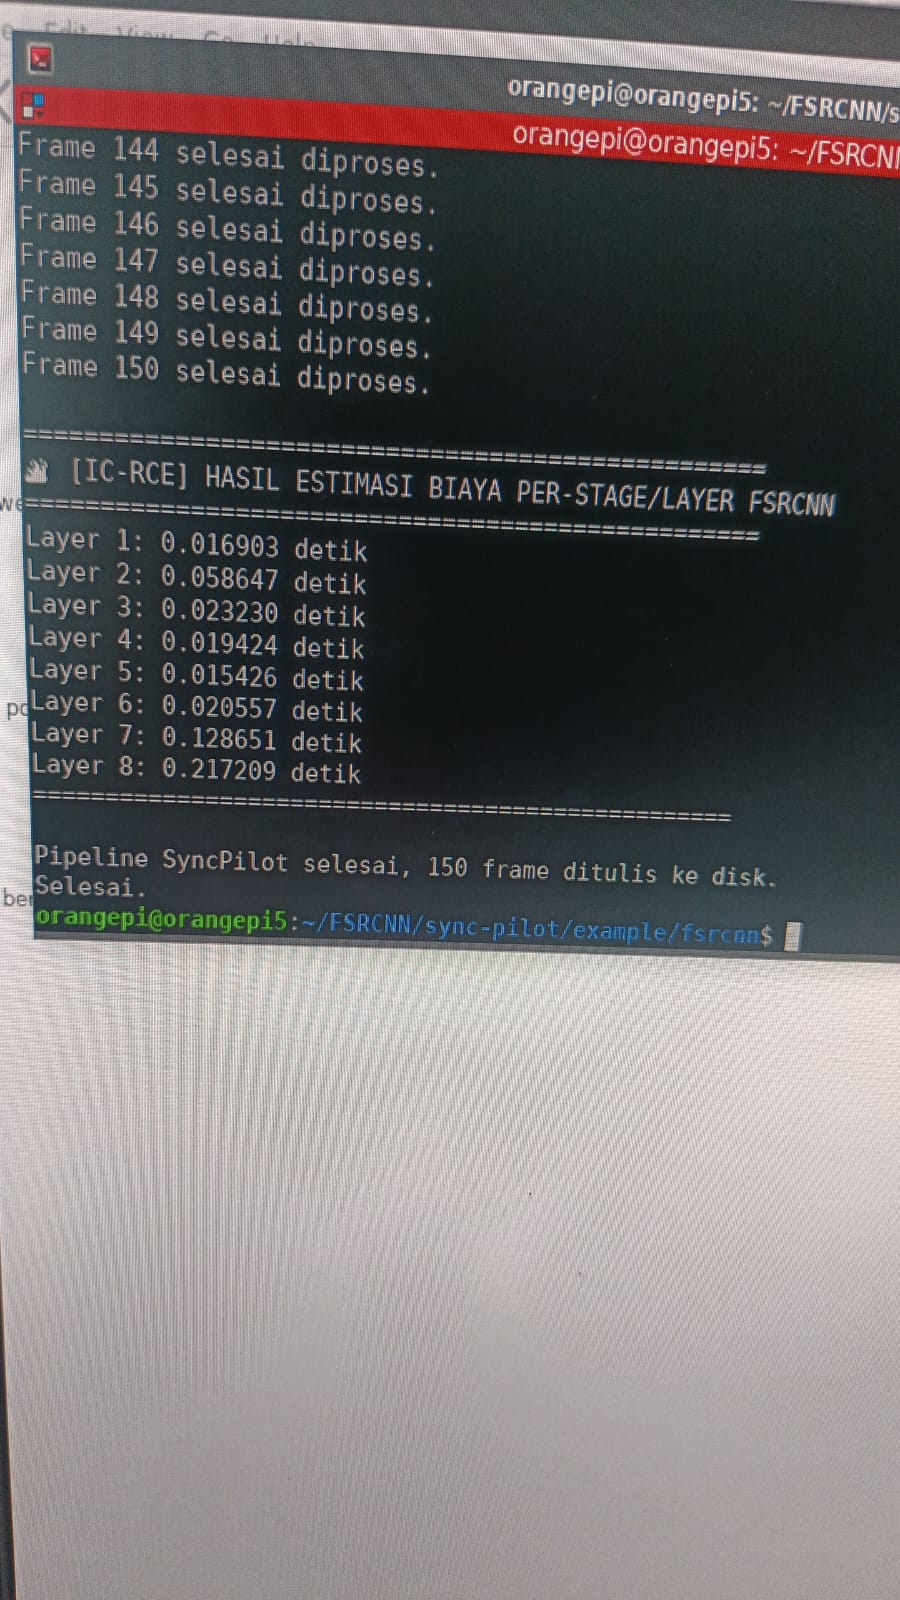
\includegraphics[width=0.9\columnwidth]{icrce_terminal_output.jpeg}
% \caption{IC-RCE output from Orange Pi 5 terminal showing per-layer cost estimation for FSRCNN. Layer 8 (deconvolution) dominates at 44.7\% of per-frame execution time.}
% \label{fig:icrce_output}
% \end{figure}

Table \ref{tab:layers} presents the IC-RCE cost table captured during the calibration phase, showing per-layer execution time for a single frame on a Big core. Layer 8 (deconvolution, $9\times9$) dominates at 44.7\% of total per-frame time (0.217s out of 0.485s), followed by Layer 7 (expanding, $1\times1$) at 26.5\%. Together, these two final stages account for 71.2\% of the per-frame cost, confirming them as the primary computational bottlenecks. This aligns with the findings in \cite{annisa2025fsrcnn}, where Layer 8 showed the lowest speedup across all parallel scenarios due to the $9\times9$ kernel requiring substantially more multiply-accumulate operations per output pixel and higher memory bandwidth demands during the upscaling from 176$\times$144 to 352$\times$288.

When scaled across the full 150-frame sequence, Layer 8's dominance translates to the aggregate execution time distribution observed in SyncPilot-4W, where the deconvolution stage consumed the majority of total execution time. This confirms that the per-frame cost profile remains consistent across the full pipeline run, validating the IC-RCE assumption that computational costs are deterministic for a fixed input resolution.

\subsection{Output Correctness Verification}
The consistency of output correctness was verified across both SyncPilot configurations and compared with the reference paper's findings. Every scenario produced output frames that were identical to the ground-truth reference, confirmed by pixel-wise comparison and infinite PSNR values. This result is significant in light of \cite{annisa2025fsrcnn}, which reported that the LITTLE CPU parallel scenario produced visible artifacts and pixel corruption due to race conditions during the deconvolution stage. SyncPilot's synchronized worker pool with reorder buffer eliminates these race conditions entirely, ensuring numerically identical outputs regardless of the worker configuration.

\subsection{Worker Configuration Analysis}
The benchmark results reveal important insights about the optimal worker configuration for asymmetric pipeline processing.

Performance consistently improves as the worker count increases on ASUS GX10. SyncPilot-4W achieves a 3.46$\times$ speedup (3016 ms), SyncPilot-8W reaches 6.61$\times$ (1581 ms), SyncPilot-10W reaches 7.83$\times$ (1334 ms), and SyncPilot-20W achieves the best performance at 9.39$\times$ (1112 ms). This scaling behavior reflects the hardware characteristics of ASUS GX10: the Cortex-A725 LITTLE cores are considerably stronger than older LITTLE core implementations, so they do not become severe stragglers when assigned heavy stages. Consequently, SyncPilot can safely exploit additional parallelism without sacrificing the critical-path performance of the deconvolution stage. This finding extends the reference paper's result \cite{annisa2025fsrcnn}, where broader worker scaling across both Big and LITTLE cores delivered the strongest gains.

\section{Discussion}

\subsection{Why Additional Workers Scale on ASUS GX10}
A counterintuitive but important finding is that on ASUS GX10, increasing the number of workers improves performance rather than degrading it. The 20-worker configuration achieves the best throughput at 1112 ms, while the 4-worker configuration trails at 3016 ms. This result reflects the hardware characteristics of ASUS GX10: the Cortex-A725 LITTLE cores are considerably stronger than the Cortex-A55 cores used on the earlier platform, so they do not become severe stragglers when assigned heavy stages. Consequently, SyncPilot can safely exploit additional parallelism without sacrificing the critical-path performance of the deconvolution stage.

\subsection{Comparison with OpenMP Affinity Approaches}
SyncPilot-20W improves over the serial baseline on ASUS GX10 by reducing the runtime from 10445 ms to 1112 ms, a 9.39$\times$ gain. This improvement comes from two key architectural differences: (1) the pull-based worker pool decouples threads from stages, allowing idle workers to proactively seek tasks rather than waiting for a specific stage's turn, and (2) the IC-RCE mechanism enables capacity-aware pulling, where Big workers preferentially select compute-intensive stages while LITTLE workers handle lighter work. The ASUS GX10 results show that, unlike the more heterogeneous platform, the stronger LITTLE cores allow the worker pool to scale far more aggressively without losing correctness or creating a severe straggler bottleneck.

\subsection{Race Condition Mitigation}
A significant finding from \cite{annisa2025fsrcnn} was that parallel FSRCNN execution on LITTLE CPUs produced visible artifacts and pixel corruption due to race conditions during the deconvolution stage. Their serial execution produced artifact-free frames, while the parallel LITTLE CPU scenario showed degraded image quality. In contrast, both SyncPilot configurations produced numerically identical outputs to the ground truth (confirmed by infinite PSNR values). This improvement stems from SyncPilot's synchronized architecture: the pull-based worker pool with shared stage queues and reorder buffer ensures that each stage's output is correctly sequenced before being consumed by the next stage, eliminating the race conditions that plagued the reference paper's OpenMP-based parallelization.

\subsection{Scalability and Limitations}
The current implementation of SyncPilot is optimized for steady-state workloads with fixed input characteristics. The IC-RCE mechanism assumes that the computational cost of each pipeline stage remains deterministic for a given input resolution. This assumption holds for FSRCNN with constant-resolution video streams (176$\times$144 $\rightarrow$ 352$\times$288), as confirmed by the low variance across steady-state runs. However, if the input workload changes drastically mid-stream (e.g., a resolution switch from 480p to 1080p), the initial calibration becomes invalid and a recalibration trigger would be required. Future work could integrate a lightweight anomaly detector to identify cost deviations and trigger a recalibration cycle, maintaining adaptability without sacrificing the low overhead of the steady-state phase.

\section{Conclusion}
We presented SyncPilot, a lightweight pipeline scheduling framework for asymmetric multicore architectures. By introducing the Initial Calibration Runtime Cost Estimation (IC-RCE), we demonstrated that efficient load balancing can be achieved without continuous runtime profiling overhead. Our evaluation on ASUS GX10 using FSRCNN for low-to-high resolution video reconstruction (176$\times$144 $\rightarrow$ 352$\times$288, Suzie sequence) shows that SyncPilot-20W achieves a 9.39$\times$ speedup (134.89 FPS, 1.112s) over the serial baseline (14.36 FPS, 10.445s). The capacity-aware worker pool design demonstrates that, on a stronger big.LITTLE platform, additional workers can be used effectively because the LITTLE cores are no longer the dominant bottleneck. Layer 8 (deconvolution) remains the dominant bottleneck, consistent with the earlier findings. All configurations produced numerically identical outputs to the ground truth (infinite PSNR), confirming that the framework maintains correctness while improving throughput. The results establish that for deterministic edge AI workloads, a one-time calibration approach combined with capacity-aware task pulling offers superior performance compared to relying solely on the OS scheduler or traditional OpenMP affinity. Future work will explore dynamic recalibration triggers for variable-resolution workloads and energy consumption measurements.

\begin{thebibliography}{16}
\bibitem{wang2020pipeit}
Wang, S., Zhou, D., Liu, Y., Zhou, X.: High-Throughput CNN Inference on Embedded ARM big.LITTLE Multicore Processors. IEEE Transactions on Computer-Aided Design of Integrated Circuits and Systems \textbf{39}(10), 1--1 (2020)

\bibitem{shi2016edge}
Shi, W., Cao, J., Zhang, Q., Li, Y., Xu, L.: Edge Computing: Vision and Challenges. IEEE Internet of Things Journal \textbf{3}(5), 637--646 (2016)

\bibitem{zhou2019edge}
Zhou, Z., Chen, X., Li, E., Zeng, K., Luo, J., Zhang, Z.: Edge Intelligence: Paving the Last Mile of Artificial Intelligence With Edge Computing. Proceedings of the IEEE \textbf{107}(8), 1738--1762 (2019)

\bibitem{green2010biglittle}
Green, D.: ARM big.LITTLE: The Future of Mobile Processing. ARM White Paper (2010)

\bibitem{arm2011biglittle}
ARM Ltd.: big.LITTLE Processing Technology. ARM Technical Reference Manual (2011)

\bibitem{leo2013cfs}
Levo, J.: Linux Completely Fair Scheduler Internals. Linux Kernel Documentation (2013)

\bibitem{curiel2017cfsamp}
Curiel, P., Knoop, K.: Understanding CFS Behavior on Heterogeneous Architectures. In: Proc. Linux Symposium, pp. 45--58 (2017)

\bibitem{cherng2014dynamicsched}
Cherng, J.-M.: Dynamic Task Scheduling for Asymmetric Multicore Processors. In: Proc. IEEE International Conference on Embedded and Real-Time Computing Systems and Applications, pp. 112--121 (2014)

\bibitem{jia2020runtimeoverhead}
Jia, T., Chen, S., Wang, J.: Runtime Profiling Overhead in Dynamic DNN Schedulers. ACM Transactions on Embedded Computing Systems \textbf{19}(4), 1--22 (2020)

\bibitem{solovyev2015pthreadaffinity}
Solovyev, I., Kuznetsov, A.: Thread Affinity Management on ARM big.LITTLE Systems. In: International Conference on Parallel and Distributed Systems (ICPADS), pp. 290--297 (2015)

\bibitem{dong2016fsrcnn}
Dong, C., Loy, C.C., Tang, X.: Accelerating the Super-Resolution Convolutional Neural Network. In: European Conference on Computer Vision (ECCV), pp. 391--407 (2016)

\bibitem{wang2021asymo}
Wang, M., Liu, S., Wang, Y.: AsyMo: Scalable and Efficient Deep-Learning Inference on Asymmetric Mobile CPUs. In: Proc. ACM MobiCom (2021)

\bibitem{yuan2025dynpipe}
Yuan, Z., Wang, X., Nie, Y., Tao, Y., Li, Y., Shao, Z., Liao, X., Li, B., Jin, H.: DynPipe: Toward Dynamic End-to-End Pipeline Parallelism for Interference-Aware DNN Training. IEEE Transactions on Parallel and Distributed Systems \textbf{36}(11), 2366--2380 (2025)

\bibitem{annisa2025fsrcnn}
Annisa, A., Adnan, Zainuddin, Z.: Enhancing computational efficiency: Transitioning from serial to parallel programming for low-to-high resolution video reconstruction using FSRCNN on AMP architecture. In: Proc. IEEE Int. Conf. Artificial Intelligence and Mechatronics Systems (AIMS), pp. 1--8 (2025). \doi{10.1109/AIMS66189.2025.11229650}

\bibitem{adnan2023array}
Adnan: Performance evaluation on work-stealing featured parallel programs on asymmetric performance multicore processors. Array \textbf{19} (2023) 100311

\bibitem{chronaki2017task}
Chronaki, K., Rico, A., Casas, M., Moretó, M., Badia, R.M., Ayguadé, E., Labarta, J., Valero, M.: Task Scheduling Techniques for Asymmetric Multi-core Systems. IEEE Transactions on Parallel and Distributed Systems \textbf{28}(7), 2074--2087 (2017)

\bibitem{saad2026qlsa}
Saad, A., Abd el-Raouf, O., Hadhoud, M., Kafafy, A.: QLSA-MOEAD: Adaptive Multi-Objective Task Scheduling in Heterogeneous Computing. Scientific Reports \textbf{16} (2026)
\end{thebibliography}

\end{document}
